

\documentclass[11pt,fleqn]{book} % Default font size and left-justified equations

%%%%%%%%%%%%%%%%%%%%%%%%%%%%%%%%%%%%%%%%%
% The Legrand Orange Book
% Structural Definitions File
% Version 2.0 (9/2/15)
%
% Original author:
% Mathias Legrand (legrand.mathias@gmail.com) with modifications by:
% Vel (vel@latextemplates.com)
% 
% This file has been downloaded from:
% http://www.LaTeXTemplates.com
%
% License:
% CC BY-NC-SA 3.0 (http://creativecommons.org/licenses/by-nc-sa/3.0/)
%
%%%%%%%%%%%%%%%%%%%%%%%%%%%%%%%%%%%%%%%%%

%----------------------------------------------------------------------------------------
%	VARIOUS REQUIRED PACKAGES AND CONFIGURATIONS
%----------------------------------------------------------------------------------------

\usepackage[top=3cm,bottom=3cm,left=5.5cm,right=3cm,headsep=10pt,letterpaper,asymmetric]{geometry} % Page margins
% Could use 6cm margin on left 

\usepackage{graphicx} % Required for including pictures
\graphicspath{{Pictures/}} % Specifies the directory where pictures are stored

\usepackage{lipsum} % Inserts dummy text

\usepackage{tikz} % Required for drawing custom shapes

\usepackage[english]{babel} % English language/hyphenation

\usepackage{enumitem} % Customize lists
\setlist{noitemsep} % Reduce spacing between bullet points and numbered lists

\usepackage{booktabs} % Required for nicer horizontal rules in tables

\usepackage{xcolor} % Required for specifying colors by name
%\definecolor{rust}{RGB}{243,102,25} % Define the orange color used for highlighting throughout the book
\definecolor{rust}{RGB}{153, 0, 0} % Define alternate red color

\usepackage{pdftexcmds}



%----------------------------------------------------------------------------------------
%	FONTS
%----------------------------------------------------------------------------------------

\usepackage{avant} % Use the Avantgarde font for headings
%\usepackage{times} % Use the Times font for headings
\usepackage{mathptmx} % Use the Adobe Times Roman as the default text font together with math symbols from the Sym­bol, Chancery and Com­puter Modern fonts

\usepackage{microtype} % Slightly tweak font spacing for aesthetics
\usepackage[utf8]{inputenc} % Required for including letters with accents
\usepackage[T1]{fontenc} % Use 8-bit encoding that has 256 glyphs
\usepackage{relsize} % Allow relative font sizing
\renewcommand\RSlargest{100pt} 
%----------------------------------------------------------------------------------------
%	BIBLIOGRAPHY AND INDEX
%----------------------------------------------------------------------------------------

\usepackage[style=alphabetic,citestyle=numeric,sorting=nyt,sortcites=true,autopunct=true,babel=hyphen,hyperref=true,abbreviate=false,backref=true,backend=biber]{biblatex}
\addbibresource{bibliography.bib} % BibTeX bibliography file
\defbibheading{bibempty}{}

\usepackage{calc} % For simpler calculation - used for spacing the index letter headings correctly
\usepackage{makeidx} % Required to make an index
\makeindex % Tells LaTeX to create the files required for indexing

%----------------------------------------------------------------------------------------
%	MAIN TABLE OF CONTENTS
%----------------------------------------------------------------------------------------

\usepackage{titletoc} % Required for manipulating the table of contents

\contentsmargin{0cm} % Removes the default margin

% Part text styling
\titlecontents{part}[0cm]
{\addvspace{20pt}\centering\large\bfseries}
{}
{}
{}

% Chapter text styling
\titlecontents{chapter}[1.25cm] % Indentation
{\addvspace{12pt}\large\sffamily\bfseries} % Spacing and font options for chapters
{\color{rust!60}\contentslabel[\Large\thecontentslabel]{1.25cm}\color{rust}} % Chapter number
{\color{rust}}  
{\color{rust!60}\normalsize\;\titlerule*[.5pc]{.}\;\thecontentspage} % Page number

% Section text styling
\titlecontents{section}[1.25cm] % Indentation
{\addvspace{3pt}\sffamily\bfseries} % Spacing and font options for sections
{\contentslabel[\thecontentslabel]{1.25cm}} % Section number
{}
{\hfill\color{black}\thecontentspage} % Page number
[]

% Subsection text styling
\titlecontents{subsection}[1.25cm] % Indentation
{\addvspace{1pt}\sffamily\small} % Spacing and font options for subsections
{\contentslabel[\thecontentslabel]{1.25cm}} % Subsection number
{}
{\ \titlerule*[.5pc]{.}\;\thecontentspage} % Page number
[]

% List of figures
\titlecontents{figure}[0em]
{\addvspace{-5pt}\sffamily}
{\thecontentslabel\hspace*{1em}}
{}
{\ \titlerule*[.5pc]{.}\;\thecontentspage}
[]

% List of tables
\titlecontents{table}[0em]
{\addvspace{-5pt}\sffamily}
{\thecontentslabel\hspace*{1em}}
{}
{\ \titlerule*[.5pc]{.}\;\thecontentspage}
[]

%----------------------------------------------------------------------------------------
%	MINI TABLE OF CONTENTS IN PART HEADS
%----------------------------------------------------------------------------------------

% Chapter text styling
\titlecontents{lchapter}[0em] % Indenting
{\addvspace{15pt}\large\sffamily\bfseries} % Spacing and font options for chapters
{\color{rust}\contentslabel[\Large\thecontentslabel]{1.25cm}\color{rust}} % Chapter number
{}  
{\color{rust}\normalsize\sffamily\bfseries\;\titlerule*[.5pc]{.}\;\thecontentspage} % Page number

% Section text styling
\titlecontents{lsection}[0em] % Indenting
{\sffamily\small} % Spacing and font options for sections
{\contentslabel[\thecontentslabel]{1.25cm}} % Section number
{}
{}

% Subsection text styling
\titlecontents{lsubsection}[.5em] % Indentation
{\normalfont\footnotesize\sffamily} % Font settings
{}
{}
{}

%----------------------------------------------------------------------------------------
%	PAGE HEADERS
%----------------------------------------------------------------------------------------

\usepackage{fancyhdr} % Required for header and footer configuration

\pagestyle{fancy}
\renewcommand{\chaptermark}[1]{\markboth{\sffamily\normalsize\bfseries\chaptername\ \thechapter.\ #1}{}} % Chapter text font settings
\renewcommand{\sectionmark}[1]{\markright{\sffamily\normalsize\thesection\hspace{5pt}#1}{}} % Section text font settings
\fancyhf{} \fancyhead[LE,RO]{\sffamily\normalsize\thepage} % Font setting for the page number in the header
\fancyhead[LO]{\rightmark} % Print the nearest section name on the left side of odd pages
\fancyhead[RE]{\leftmark} % Print the current chapter name on the right side of even pages
\renewcommand{\headrulewidth}{0.5pt} % Width of the rule under the header
\addtolength{\headheight}{2.5pt} % Increase the spacing around the header slightly
\renewcommand{\footrulewidth}{0pt} % Removes the rule in the footer
\fancypagestyle{plain}{\fancyhead{}\renewcommand{\headrulewidth}{0pt}} % Style for when a plain pagestyle is specified

% Removes the header from odd empty pages at the end of chapters
\makeatletter
\renewcommand{\cleardoublepage}{
\clearpage\ifodd\c@page\else
\hbox{}
\vspace*{\fill}
\thispagestyle{empty}
\newpage
\fi}

%----------------------------------------------------------------------------------------
%	THEOREM STYLES
%----------------------------------------------------------------------------------------

\usepackage{amsmath,amsfonts,amssymb,amsthm} % For math equations, theorems, symbols, etc

\newcommand{\intoo}[2]{\mathopen{]}#1\,;#2\mathclose{[}}
\newcommand{\ud}{\mathop{\mathrm{{}d}}\mathopen{}}
\newcommand{\intff}[2]{\mathopen{[}#1\,;#2\mathclose{]}}
\newtheorem{notation}{Notation}[chapter]

% Boxed/framed environments
\newtheoremstyle{rustnumbox}% % Theorem style name
{0pt}% Space above
{0pt}% Space below
{\normalfont}% % Body font
{}% Indent amount
{\small\bf\sffamily\color{rust}}% % Theorem head font
{\;}% Punctuation after theorem head
{0.25em}% Space after theorem head
{\small\sffamily\color{rust}\thmname{#1}\nobreakspace\thmnumber{\@ifnotempty{#1}{}\@upn{#2}}% Theorem text (e.g. Theorem 2.1)
\thmnote{\nobreakspace\the\thm@notefont\sffamily\bfseries\color{black}---\nobreakspace#3.}} % Optional theorem note
\renewcommand{\qedsymbol}{$\blacksquare$}% Optional qed square

\newtheoremstyle{blacknumex}% Theorem style name
{5pt}% Space above
{5pt}% Space below
{\normalfont}% Body font
{} % Indent amount
{\small\bf\sffamily}% Theorem head font
{\;}% Punctuation after theorem head
{0.25em}% Space after theorem head
{\small\sffamily{\tiny\ensuremath{\blacksquare}}\nobreakspace\thmname{#1}\nobreakspace\thmnumber{\@ifnotempty{#1}{}\@upn{#2}}% Theorem text (e.g. Theorem 2.1)
\thmnote{\nobreakspace\the\thm@notefont\sffamily\bfseries---\nobreakspace#3.}}% Optional theorem note

\newtheoremstyle{blacknumbox} % Theorem style name
{0pt}% Space above
{0pt}% Space below
{\normalfont}% Body font
{}% Indent amount
{\small\bf\sffamily}% Theorem head font
{\;}% Punctuation after theorem head
{0.25em}% Space after theorem head
{\small\sffamily\thmname{#1}\nobreakspace\thmnumber{\@ifnotempty{#1}{}\@upn{#2}}% Theorem text (e.g. Theorem 2.1)
\thmnote{\nobreakspace\the\thm@notefont\sffamily\bfseries---\nobreakspace#3.}}% Optional theorem note

% Non-boxed/non-framed environments
\newtheoremstyle{rustnum}% % Theorem style name
{5pt}% Space above
{5pt}% Space below
{\normalfont}% % Body font
{}% Indent amount
{\small\bf\sffamily\color{rust}}% % Theorem head font
{\;}% Punctuation after theorem head
{0.25em}% Space after theorem head
{\small\sffamily\color{rust}\thmname{#1}\nobreakspace\thmnumber{\@ifnotempty{#1}{}\@upn{#2}}% Theorem text (e.g. Theorem 2.1)
\thmnote{\nobreakspace\the\thm@notefont\sffamily\bfseries\color{black}---\nobreakspace#3.}} % Optional theorem note
\renewcommand{\qedsymbol}{$\blacksquare$}% Optional qed square
\makeatother

% Defines the theorem text style for each type of theorem to one of the three styles above
\newcounter{dummy} 
\numberwithin{dummy}{section}
\theoremstyle{rustnumbox}
\newtheorem{theoremeT}[dummy]{Theorem}
\newtheorem{assignment}{Assignment}[chapter]

\newtheorem{exerciseT}{Exercise}[chapter]
\theoremstyle{blacknumex}
\newtheorem{exampleT}{Example}[chapter]
\theoremstyle{blacknumbox}
\newtheorem{vocabulary}{Vocabulary}[chapter]
\newtheorem{definitionT}{Definition}[section]
\newtheorem{corollaryT}[dummy]{Corollary}
\theoremstyle{rustnum}
\newtheorem{proposition}[dummy]{Proposition}

%----------------------------------------------------------------------------------------
%	DEFINITION OF COLORED BOXES
%----------------------------------------------------------------------------------------

\RequirePackage[framemethod=default]{mdframed} % Required for creating the theorem, definition, exercise and corollary boxes

% Theorem box
\newmdenv[skipabove=7pt,
skipbelow=7pt,
backgroundcolor=black!5,
linecolor=rust,
innerleftmargin=5pt,
innerrightmargin=5pt,
innertopmargin=5pt,
leftmargin=0cm,
rightmargin=0cm,
innerbottommargin=5pt]{tBox}

% Exercise box	  
\newmdenv[skipabove=7pt,
skipbelow=7pt,
rightline=false,
leftline=true,
topline=false,
bottomline=false,
backgroundcolor=rust!10,
linecolor=rust,
innerleftmargin=5pt,
innerrightmargin=5pt,
innertopmargin=5pt,
innerbottommargin=5pt,
leftmargin=0cm,
rightmargin=0cm,
linewidth=4pt]{eBox}	

% Definition box
\newmdenv[skipabove=7pt,
skipbelow=7pt,
rightline=false,
leftline=true,
topline=false,
bottomline=false,
linecolor=rust,
innerleftmargin=5pt,
innerrightmargin=5pt,
innertopmargin=0pt,
leftmargin=0cm,
rightmargin=0cm,
linewidth=4pt,
innerbottommargin=0pt]{dBox}	

% Corollary box
\newmdenv[skipabove=7pt,
skipbelow=7pt,
rightline=false,
leftline=true,
topline=false,
bottomline=false,
linecolor=gray,
backgroundcolor=black!5,
innerleftmargin=5pt,
innerrightmargin=5pt,
innertopmargin=5pt,
leftmargin=0cm,
rightmargin=0cm,
linewidth=4pt,
innerbottommargin=5pt]{cBox}

% Creates an environment for each type of theorem and assigns it a theorem text style from the "Theorem Styles" section above and a colored box from above
\newenvironment{theorem}{\begin{tBox}\begin{theoremeT}}{\end{theoremeT}\end{tBox}}
\newenvironment{exercise}{\begin{eBox}\begin{exerciseT}}{\hfill{\color{rust}\tiny\ensuremath{\blacksquare}}\end{exerciseT}\end{eBox}}				  
\newenvironment{definition}{\begin{dBox}\begin{definitionT}}{\end{definitionT}\end{dBox}}	
\newenvironment{example}{\begin{exampleT}}{\hfill{\tiny\ensuremath{\blacksquare}}\end{exampleT}}		
\newenvironment{corollary}{\begin{cBox}\begin{corollaryT}}{\end{corollaryT}\end{cBox}}	

%----------------------------------------------------------------------------------------
%	WARNING ENVIRONMENT
%----------------------------------------------------------------------------------------

\newenvironment{warning}{\par\vspace{10pt}\small % Vertical white space above the remark and smaller font size
	\begin{list}{}{
			\leftmargin=35pt % Indentation on the left
			\rightmargin=25pt}\item\ignorespaces % Indentation on the right
		\makebox[-2.5pt]{\begin{tikzpicture}[overlay]
			\node[draw=rust!60,line width=1pt,circle,fill=rust!25,font=\sffamily\bfseries,inner sep=2pt,outer sep=0pt] at (-15pt,0pt){\textcolor{rust}{\textbf{!}}};\end{tikzpicture}} 
		\advance\baselineskip -1pt}{\end{list}\vskip5pt} % Tighter line spacing and white space after remark

%----------------------------------------------------------------------------------------
%	REMARK ENVIRONMENT
%----------------------------------------------------------------------------------------

\newenvironment{remark}{\par\vspace{10pt}\small % Vertical white space above the remark and smaller font size
\begin{list}{}{
\leftmargin=35pt % Indentation on the left
\rightmargin=25pt}\item\ignorespaces % Indentation on the right
\makebox[-2.5pt]{\begin{tikzpicture}[overlay]
\node[draw=rust!60,line width=1pt,circle,fill=rust!25,font=\sffamily\bfseries,inner sep=2pt,outer sep=0pt] at (-15pt,0pt){\textcolor{rust}{R}};\end{tikzpicture}} % Orange R in a circle
\advance\baselineskip -1pt}{\end{list}\vskip5pt} % Tighter line spacing and white space after remark

%----------------------------------------------------------------------------------------
%	SECTION NUMBERING IN THE MARGIN
%----------------------------------------------------------------------------------------

\makeatletter

% just bottom line
%\newmdenv[topline=false,leftline=false,rightline=false]{test123}

%\newmdenv[
%rightline=false, leftline=false, topline=false, bottomline=true,
%linecolor=rust, linewidth=4pt
%]{sectionUnderline}

% Adjusts all numbering for sections and subsections
\renewcommand{\@seccntformat}[1]{  
    \ifnum\pdf@strcmp{#1}{section}=\z@ 
    
    %\llap{\colorbox{gray!15}{\makebox[3.25cm][r]{\textcolor{gray}{\textsc{\@nameuse{secTypeName}}\hspace{0.5em}\relsize{1.25}\textcolor{rust}{\csname the#1\endcsname}}}}\hspace{.5em}}
    \llap{
        %\begin{sectionUnderline}
            \makebox[3.25cm][r]{\textcolor{gray}{\textsc{\@nameuse{secTypeName}}\hspace{0.5em}\relsize{1.25}\textcolor{rust}{\csname the#1\endcsname}}}
            \textcolor{rust}{\hspace{-3.25cm}\rule[-.2cm]{3.13cm}{2pt}}
        %\end{sectionUnderline}
        \hspace{.5em}
    }
    \else
    \llap{\textcolor{rust}{\csname the#1\endcsname}\hspace{1em}}%
    \fi 
   % \llap{\textcolor{rust}{\csname the#1\endcsname}\hspace{1em}}
}  % hspace controls spacing of section number to section name    


\newcommand{\setSectionType}[1]{
    \@namedef{secTypeName}{#1}
}
        
\renewcommand{\section}{\@startsection{section}{1}{-8pt}
{-5ex \@plus -1ex \@minus -.2ex}
{2.0ex \@plus.2ex }
{\normalfont\large\sffamily\bfseries}}


\renewcommand{\subsection}{\@startsection {subsection}{2}{-3pt}
{-3ex \@plus -0.1ex \@minus -.4ex}
{0.5ex \@plus.2ex }
{\normalfont\sffamily\bfseries}}
\renewcommand{\subsubsection}{\@startsection {subsubsection}{3}{\z@}
{-2ex \@plus -0.1ex \@minus -.2ex}
{.2ex \@plus.2ex }
{\normalfont\small\sffamily\bfseries}}                        
\renewcommand\paragraph{\@startsection{paragraph}{4}{\z@}
{-2ex \@plus-.2ex \@minus .2ex}
{.1ex}
{\normalfont\small\sffamily\bfseries}}

%----------------------------------------------------------------------------------------
%	PART HEADINGS
%----------------------------------------------------------------------------------------

% numbered part in the table of contents
\newcommand{\@mypartnumtocformat}[2]{%
\setlength\fboxsep{0pt}%
\noindent\colorbox{rust!20}{\strut\parbox[c][.7cm]{\ecart}{\color{rust!70}\Large\sffamily\bfseries\centering#1}}\hskip\esp\colorbox{rust!40}{\strut\parbox[c][.7cm]{\linewidth-\ecart-\esp}{\Large\sffamily\centering#2}}}%
%%%%%%%%%%%%%%%%%%%%%%%%%%%%%%%%%%
% unnumbered part in the table of contents
\newcommand{\@myparttocformat}[1]{%
\setlength\fboxsep{0pt}%
\noindent\colorbox{rust!40}{\strut\parbox[c][.7cm]{\linewidth}{\Large\sffamily\centering#1}}}%
%%%%%%%%%%%%%%%%%%%%%%%%%%%%%%%%%%
\newlength\esp
\setlength\esp{4pt}
\newlength\ecart
\setlength\ecart{1.2cm-\esp}
\newcommand{\thepartimage}{}%
\newcommand{\partimage}[1]{\renewcommand{\thepartimage}{#1}}%
\def\@part[#1]#2{%
\ifnum \c@secnumdepth >-2\relax%
\refstepcounter{part}%
\addcontentsline{toc}{part}{\texorpdfstring{\protect\@mypartnumtocformat{\thepart}{#1}}{\partname~\thepart\ ---\ #1}}
\else%
\addcontentsline{toc}{part}{\texorpdfstring{\protect\@myparttocformat{#1}}{#1}}%
\fi%
\startcontents%
\markboth{}{}%
{\thispagestyle{empty}%
\begin{tikzpicture}[remember picture,overlay]%
\node at (current page.north west){\begin{tikzpicture}[remember picture,overlay]%	
\node[anchor=north] at (4cm,-3.25cm){\color{rust!60}\fontsize{220}{100}\sffamily\bfseries\@Roman\c@part}; 
\node[anchor=south east] at (\paperwidth-1cm,-\paperheight+1cm){\parbox[t][][t]{8.5cm}{
\printcontents{l}{0}{\setcounter{tocdepth}{1}}%
}};
\node[anchor=north east] at (\paperwidth-1.5cm,-3.25cm){\parbox[t][][t]{15cm}{\strut\raggedleft\color{black!40}\fontsize{30}{30}\sffamily\bfseries#2}};
\end{tikzpicture}};
\end{tikzpicture}}%
\@endpart}
\def\@spart#1{%
\startcontents%
\phantomsection
{\thispagestyle{empty}%
\begin{tikzpicture}[remember picture,overlay]%
\node at (current page.north west){\begin{tikzpicture}[remember picture,overlay]%	
\fill[rust!20](0cm,0cm) rectangle (\paperwidth,-\paperheight);
\node[anchor=north east] at (\paperwidth-1.5cm,-3.25cm){\parbox[t][][t]{15cm}{\strut\raggedleft\color{white}\fontsize{30}{30}\sffamily\bfseries#1}};
\end{tikzpicture}};
\end{tikzpicture}}
\addcontentsline{toc}{part}{\texorpdfstring{%
\setlength\fboxsep{0pt}%
\noindent\protect\colorbox{rust!40}{\strut\protect\parbox[c][.7cm]{\linewidth}{\Large\sffamily\protect\centering #1\quad\mbox{}}}}{#1}}%
\@endpart}
\def\@endpart{\vfil\newpage
\if@twoside
\if@openright
\null
\thispagestyle{empty}%
\newpage
\fi
\fi
\if@tempswa
\twocolumn
\fi}

%----------------------------------------------------------------------------------------
%	CHAPTER HEADINGS
%----------------------------------------------------------------------------------------

% A switch to conditionally include a picture, implemented by  Christian Hupfer
\newif\ifusechapterimage
\usechapterimagetrue
\newcommand{\thechapterimage}{}%
\newcommand{\chapterimage}[1]{\ifusechapterimage\renewcommand{\thechapterimage}{#1}\fi}%
\def\@makechapterhead#1{%
{\parindent \z@ \raggedright \normalfont
\ifnum \c@secnumdepth >\m@ne
\if@mainmatter
\begin{tikzpicture}[remember picture,overlay]
\node at (current page.north west)
{\begin{tikzpicture}[remember picture,overlay]
\node[anchor=north west,inner sep=0pt] at (0,0) {\ifusechapterimage\includegraphics[width=\paperwidth]{\thechapterimage}\fi};
%\draw[anchor=west] (\Gm@lmargin,-9cm) node [line width=2pt,rounded corners=15pt,draw=rust,fill=white,fill opacity=0.5,inner sep=15pt]{\strut\makebox[22cm]{}};

%%%%% Chapter text sizing
%\draw[anchor=west] (\Gm@lmargin-1.3cm,-4cm) node [line width=2pt,rounded corners=15pt,draw=rust,fill=white,fill opacity=0.75,inner sep=15pt]{\strut\makebox[22cm]{}};

%\draw[anchor=west] (\Gm@lmargin-1cm,-4.1cm) node {\huge\sffamily\bfseries\color{black}\thechapter. #1\strut};

% Use larger chapter number

\draw[anchor=west] (\Gm@lmargin-1.3cm,-3.9cm) node [line width=2pt,rounded corners=8pt,draw=rust,fill=white,fill opacity=0.75,inner sep=15pt]{\strut\makebox[22cm]{}};

\draw[anchor=west] (\Gm@lmargin-1cm,-4.0cm) node {\huge\sffamily\bfseries\color{black}{\relsize{2}\thechapter. }#1\strut};


\end{tikzpicture}};
\end{tikzpicture}
\else
\begin{tikzpicture}[remember picture,overlay]
\node at (current page.north west)
{\begin{tikzpicture}[remember picture,overlay]
\node[anchor=north west,inner sep=0pt] at (0,0) {\ifusechapterimage\includegraphics[width=\paperwidth]{\thechapterimage}\fi};
%\draw[anchor=west] (\Gm@lmargin,-9cm) node [line width=2pt,rounded corners=15pt,draw=rust,fill=white,fill opacity=0.5,inner sep=15pt]{\strut\makebox[22cm]{}};

\draw[anchor=west] (\Gm@lmargin,-4cm) node [line width=2pt,rounded corners=15pt,draw=rust,fill=white,fill opacity=0.75,inner sep=15pt]{\strut\makebox[22cm]{}};

\draw[anchor=west] (\Gm@lmargin+.3cm,-4cm) node {\huge\sffamily\bfseries\color{black}#1\strut};
\end{tikzpicture}};
\end{tikzpicture}
%\fi\fi\par\vspace*{270\p@}}}

\fi\fi\par\vspace*{150\p@}}}

%-------------------------------------------

\def\@makeschapterhead#1{%
\begin{tikzpicture}[remember picture,overlay]
\node at (current page.north west)
{\begin{tikzpicture}[remember picture,overlay]
\node[anchor=north west,inner sep=0pt] at (0,0) {\ifusechapterimage\includegraphics[width=\paperwidth]{\thechapterimage}\fi};
\draw[anchor=west] (\Gm@lmargin,-9cm) node [line width=2pt,rounded corners=15pt,draw=rust,fill=white,fill opacity=0.5,inner sep=15pt]{\strut\makebox[22cm]{}};
\draw[anchor=west] (\Gm@lmargin+.3cm,-9cm) node {\huge\sffamily\bfseries\color{black}#1\strut};
\end{tikzpicture}};
\end{tikzpicture}
\par\vspace*{270\p@}}
\makeatother

%----------------------------------------------------------------------------------------
%	HYPERLINKS IN THE DOCUMENTS
%----------------------------------------------------------------------------------------

\usepackage{hyperref}
\hypersetup{hidelinks,backref=true,pagebackref=true,hyperindex=true,colorlinks=false,breaklinks=true,urlcolor= rust,bookmarks=true,bookmarksopen=false,pdftitle={Lab Manual},pdfauthor={Brent Mellor}}
\usepackage{bookmark}
\bookmarksetup{
open,
numbered,
addtohook={%
\ifnum\bookmarkget{level}=0 % chapter
\bookmarksetup{bold}%
\fi
\ifnum\bookmarkget{level}=-1 % part
\bookmarksetup{color=rust,bold}%
\fi
}
}
 % Insert the commands.tex file which contains the majority of the structure behind the template
\usepackage{float}

\usepackage{amsmath}

\usepackage{listings} 
\lstset
{ 
    language=C,
    basicstyle=\ttfamily,
    columns=fullflexible,
    keepspaces=true,
    numbers=none,
    stepnumber=1,
    showstringspaces=false,
    tabsize=1,
    breaklines=true,
    breakatwhitespace=false,
    keywordstyle=\color{blue!80!black},
    stringstyle=\color{red!80!black},
    commentstyle=\color{green!40!black},
    morecomment=[l][\color{magenta!80!black}]{\#}
}

\usepackage{caption}
\captionsetup[figure]{font=small,skip=10pt}

%\usepackage{enumitem}
%\setlist{noitemsep} % or \setlist{noitemsep} to leave space around whole list


%%%%% May be too harsh to prevent paragraph breaks across pages! 
%\interlinepenalty 10000
\widowpenalties 1 10000
\raggedbottom


\newcommand{\ilcode}[1]{
    %\vspace{0.5pt}
    \smallskip
    \colorbox{gray!20!white}{
        \centering
        \parbox{\linewidth-2\fboxsep}{
            \lstinline@#1@
        }
    }
    %\vspace{0.5pt}
}

\newcommand{\code}[3]{
    \begin{figure}[]
        \colorbox{gray!20!white}{
            \parbox{\linewidth-2\fboxsep} {
                \centering 
                \lstinputlisting[language=C]{#1}
            }
        }
        \caption{#2}
        \label{#3}
    \end{figure}
}


%\begin{figure}[]
%    \centering\includegraphics[width=0.75\textwidth]{}
%    \caption{}
%    \label{}
%\end{figure}

\usepackage{textcomp}
\usepackage{wrapfig}
\usepackage{float}

\usepackage{silence} % http://ctan.org/pkg/silence
\ErrorFilter{textcomp}{Symbol \textrightarrow not provided}

% Disable paragraph indentation globally since template was indenting some and not others. (looked terrible)
\setlength{\parindent}{0pt}


%%%%%%%%%%%%%%%%%%%%%%%%%%%%%%%%%%%%%%%%%%%%%%%%%%%%%%%%%%%%%%%%%%%%%%%%%%%%%%%%%%%%%%%%%%%%%%%%%
%%%%                                                                                         %%%%
%%%%       Chapter 4: Timers, PWM and GPIO Alternate Functions                               %%%%
%%%%                                                                                         %%%%
%%%%%%%%%%%%%%%%%%%%%%%%%%%%%%%%%%%%%%%%%%%%%%%%%%%%%%%%%%%%%%%%%%%%%%%%%%%%%%%%%%%%%%%%%%%%%%%%%

\setcounter{chapter}{3} % Manually adjust chapter counter to number before desired chapter heading

\begin{document}
	
\chapterimage{chapter_head_2.png} % Chapter heading image
\chapter{Timers, PWM and GPIO Alternate Functions}

\section{Introduction to Timers}
The last lab used the SysTick timer to generate a periodic interrupt. The SysTick is a simple peripheral with a 24-bit down-counting register that triggers an interrupt as it reaches zero. The primary purpose of the SysTick timer is to generate a stable system ``tick'' or heartbeat/timing reference signal. 

This heartbeat signal is used to indicate the passage of a unit of time. Some common places where the SysTick is used is in the HAL delay libraries and in the context switcher of real-time operating systems. 

An interesting question to ask is why accurate timing so important. Although a processor moves along an applications code in units of the clock cycle, it is difficult and inefficient to measure time simply by counting instruction cycles without dedicated hardware such as a timer. The requirement for accurate timing stems from the fact that many embedded systems require specific timings or schedules while interacting with the physical world.

Timers are at their core simply a register the increments or decrements whenever a trigger signal occurs. Upon this are built the capability to generate hardware interrupts, like the SysTick. However, the SysTick is the simplest of the onboard timer peripherals.
    
    \subsection{Systick vs Peripheral Timers}
     Because the SysTick peripheral has a very simple purpose, to generate periodic interrupts, it doesn't offer any features that make it useful for more complicated tasks. 
     
     Unlike the SysTick, peripheral timers within the STM32F0 are designed to be useful in whatever tasks the user application requires. Because of this, they are relatively complicated devices with a large variety of features. Figure \ref{block_timers} shows the block diagram for general-purpose timers 2 \& 3 in the STM32F072.  

        \begin{figure}[]
            \centering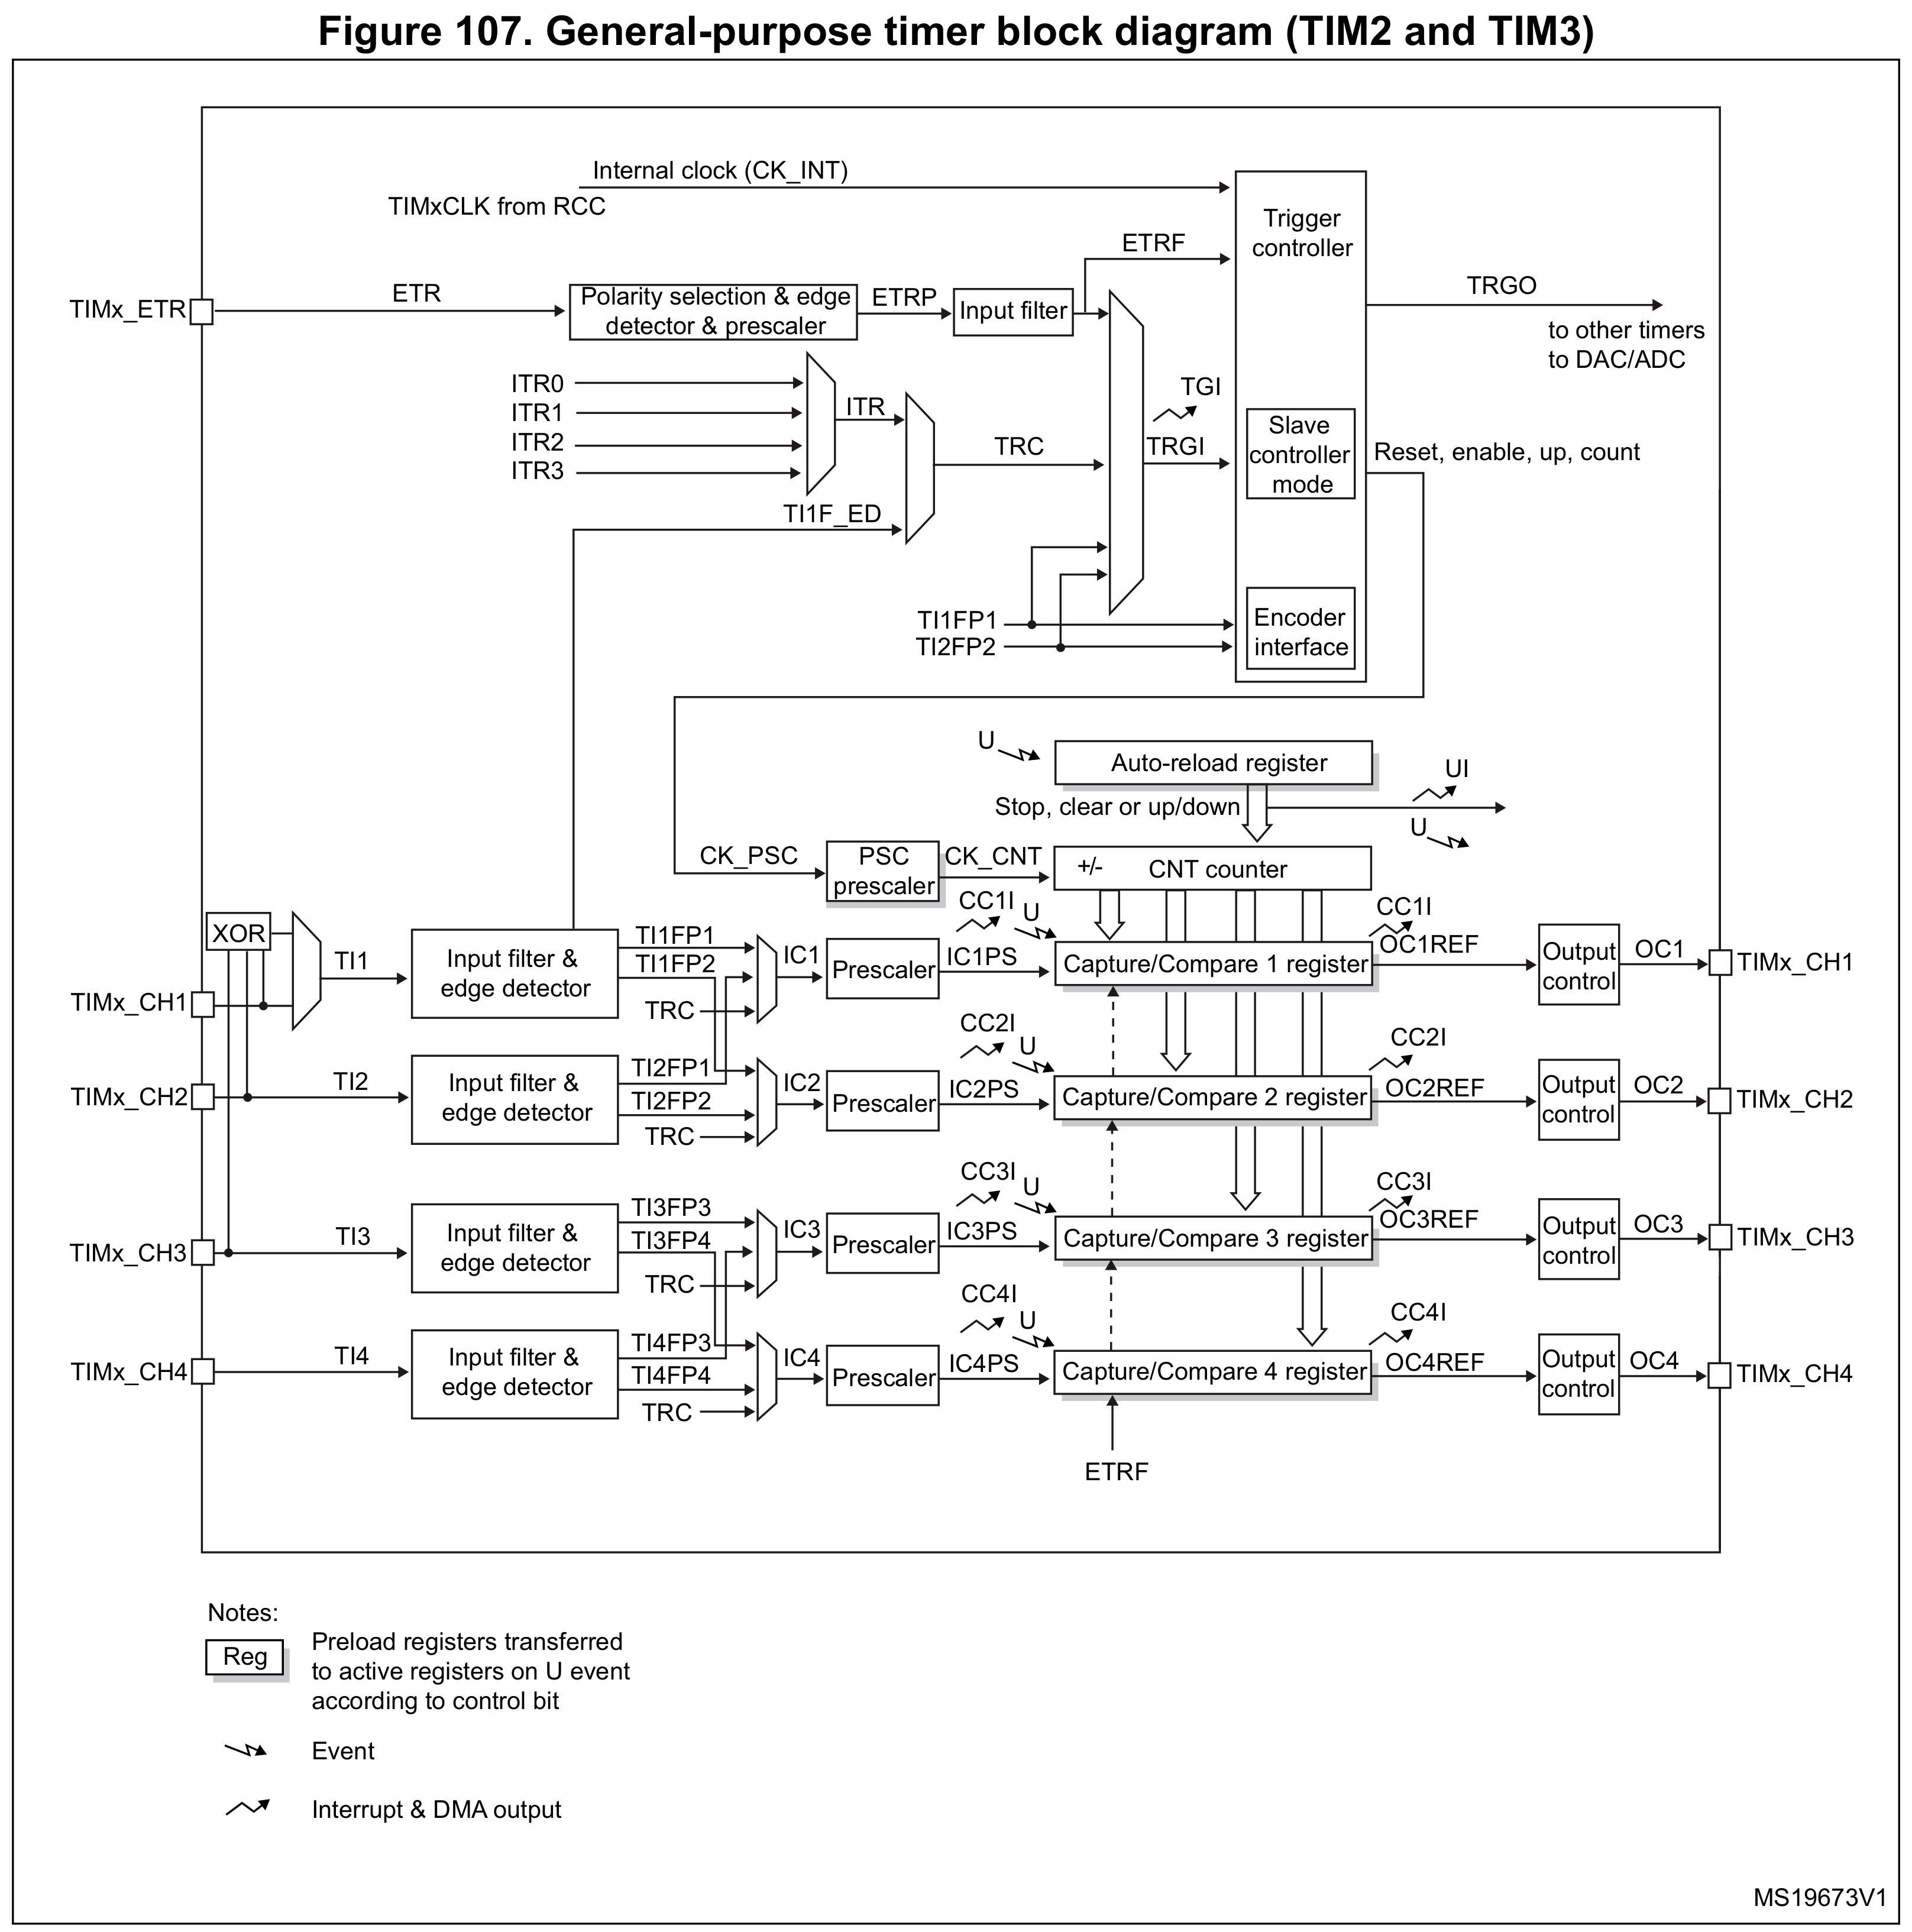
\includegraphics[width=\textwidth]{block_timers}
            \caption{Block diagram of timers 2 \& 3}
            \label{block_timers}
        \end{figure}
        
        The three main features that peripheral timers offer over simpler devices such as the SysTick are:
        \begin{enumerate}
            \item \textbf{Selectable and Prescalable Clock Sources} -- Many peripheral timers can use multiple signals as clock sources and can divide the input frequency by arbitrary integer values. 
            \item \textbf{Generate Interrupts at Multiple Conditions} -- Many peripheral timers can generate interrupts at arbitrary counter values.
            \item \textbf{Directly Modify GPIO Pins} -- Many peripheral timers can directly set or capture GPIO pin states to measure or generate digital signals.  
        \end{enumerate}
        
	
    
    \subsection{Timers in the STM32F072}
        %(Show table of timers in the STM32F072)
        \begin{figure}[]
            \centering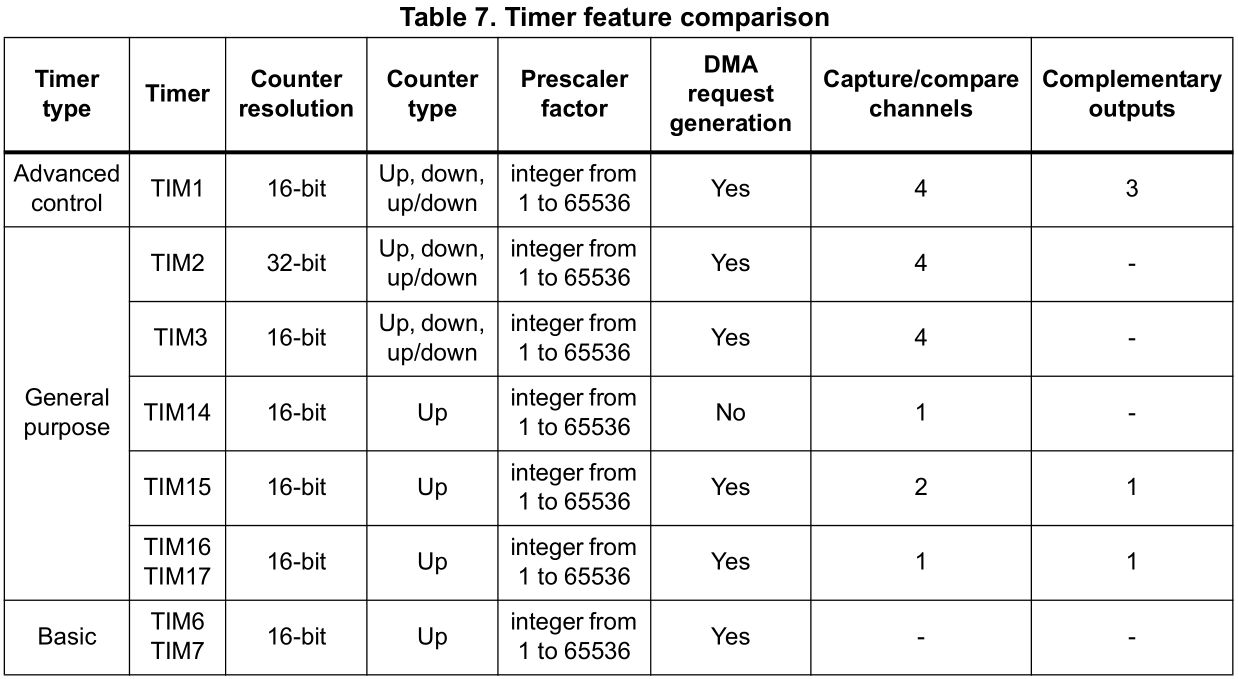
\includegraphics[width=\textwidth]{avaliable_timers}
            \caption{STM32F072RB hardware timers}
            \label{avaliable_timers}
        \end{figure}
        
        
        Figure \ref{avaliable_timers} shows the timers available in the STM32F072 chip we are using. When deciding on a timer to use for an application, it is helpful to understand their capabilities and if they are suitable for the task. A brief breakdown of the information in figure \ref{avaliable_timers} is as follows:
        
        \begin{itemize}
            \item \textbf{Timer Type} -- There are multiple classes of timers within the STM32F0. These serve as indicators of the appropriate uses for the peripheral. An advanced control timer offers additional and more complex operating modes than a general-purpose one. 
            \item \textbf{Timer} -- These abbreviated names are used to identify between timers in the documentation. They are also the defined names for the timer structures in the supporting peripheral header files. 
            \item \textbf{Counter Resolution} -- This indicates how large the hardware counter within the timer is. A 16-bit timer can only count to $2^{16}$ values before overflowing and wrapping back to zero. 
            \item \textbf{Counter Type} -- Typically the hardware counter in a timer counts upwards with each clock cycle. However, more advanced timers can also be set to count downwards from a value or to change direction whenever reaching the limit values automatically. 
            \item \textbf{Prescaler Factor} -- The prescale factor allows the timer to pre-divide the input clock to a slower frequency. The timers within the STM32F0 have the ability to divide the input clock by arbitrary integer factors between 1 and $2^{16}$.
            \item \textbf{DMA Request Generation} -- Many peripherals have the ability to move data between peripheral registers and system memory without using the processor. This process is called direct memory access (DMA).
            \item \textbf{Capture/Compare Channels} -- Most timers have the ability to modify GPIO pins without using the GPIO peripheral directly. The capture/compare system in a timer is used to generate and measure digital signals on an external pin. 
            \item \textbf{Complementary Outputs} -- The capture/compare circuity in some timers can generate complementary or opposing outputs on two GPIO pins. 
        \end{itemize}

\section{Using the Timer Documentation}
    At this point, the peripherals that the labs are going to be discussing are going to be reaching the level of complexity that the lab manuals are not going to be able to provide enough information to complete the lab assignments without additional reading in the datasheets and peripheral reference manual. 
    
    Instead, this lab manual will provide an overview of the different modes of operation and their relevant registers within the peripheral.

    In figure \ref{avaliable_timers} we discussed the characteristics of the available timers in the STM32F072. For the remainder of this lab manual, we will be focusing on the documentation materials for TIM2 \& TIM3. 
    
    Timers 2 \& 3 are the more-advanced versions of the general purpose timers in the STM32F0. Although not as complex as the advanced control timer 1, they feature additional configuration options and more output channels. Because these have a nearly identical interface as the simpler timers, by reading through their documentation, you should be able to move to one of the simpler devices without trouble in the assignment. 
    
    \subsubsection{Organization of Peripheral Documentation}
    The each section of the peripheral reference manual follows a similar organization regardless of the peripheral documented. These begin with a brief introduction of the purpose and features of the peripheral, followed by a block diagram showing the basic architectural design of the hardware. 
    
    The following section titled the \textit{Functional Description} is the most important piece of material that you will use when figuring out a new peripheral. The functional description section of the manual provides the following information:
    
    \begin{itemize}
        \item Explanation of the purpose of each operating mode 
        \item Basic theory of operation 
        \item Relevant registers and configuration options 
        \item Summarized configuration information
        \begin{itemize}
            \item Typically provides generic steps for peripheral configuration. 
            \item These provide a foundation when searching the register documentation for additional details. 
        \end{itemize}
        \item Summary of the output data produced
        \begin{itemize}
            \item Indicates where data is written for application use.
            \item Typically includes figures and graphs depicting peripheral operation.
        \end{itemize}
    \end{itemize}

    After the functional description, the reference manual documents each of the peripheral's registers in detail. Assuming that you have read and understand the information within the functional description section, you will spend the majority of your time using the register maps and bit descriptions to configure the peripheral into the desired behavior. 

%    The following sections will attempt to provide a summarized version of the important information in the functional description for the timer 2 \& 3 peripherals. 
%        Their documentation is 65 pages long... (and dense)
%    
%    Reference manual documentation goes in this format:
%        Basic information on what peripheral does
%        Details and architectural block diagrams
%        Documentation of the different modes
%        These usually have some specific background info
%        Summarized information on how to configure the mode
%            Gives generic steps, will need to carefully read the register documentation
%        Summarized information on data produced 
%            describe where produced data is written
%            Includes figures depicting operation
%    
%    This manual will document the purpose of the base registers as they are used in each mode
%        May also indicate groups of control bits that pertain to the configuration or operation 	

\section{Using Timers to Generate Interrupts and Events} \label{timer_interrupts}

    One of the most basic uses of a timer is to generate periodic interrupts. Unlike the SysTick timer which is typically configured once and to a specific base unit of time, the peripheral timers are available to use with arbitrary timing periods and can be utilized as event counters when using other signals as clock sources. Because their input prescaler can be used to divide the input clock by arbitrary integer values, it is possible to generate very long timer periods or match strange timing requirements that aren't multiples of the system clock. Section 18.3 \textit{TIM2 and TIM3 Functional Description} of the peripheral reference manual documents the following sections in greater detail. 
    
    Three registers form the core operations of a timer peripheral. 
    \subsubsection{Timer Counter Register (CNT)}
    The CNT register holds the current value of the counter in the timer. Its size depends on the counter resolution (16/32-bit) indicated in the timer's documentation. Although this register is automatically updated as the timer operates, it is possible to read and edit its value manually. The CNT register can be read within the main application loop as a method of counting time or written to modify the timer's operation. 
    \subsubsection{Timer Prescaler Register (PSC)}
    The PSC register is used to divide the input clock frequency to the timer. It is value is 0-indexed meaning that a value of 0 in the PSC register divides the clock source by 1. (no frequency scaling) Likewise a value of 1 in the PSC register divides the clock source by 2 and causes the timer to count at half the clock frequency. The PSC can divide the input clock by any integer value that fits in its 16-bit width.  
    \subsubsection{Timer Auto-Reload Register (ARR)}
     Although a timer has a physical hardware size to its counter register, it is possible to set an artificial top limit. The value in the ARR register is the trigger point where the timer resets and begins to count a new period. The actual behavior of the timer depends on its counting mode and is discussed more in a later section. 

    
    \subsection{Basic Timer Operation}
    
    There are three different counting modes that the timers can operate under; up, down, and center-aligned (up/down). Note that all but three of the hardware timers in the STM32F072 are only upcounters. Figure \ref{count_modes} shows a graphical representation of the counting modes.  
    
    \begin{itemize}
        \item \textbf{Upcounting Mode} --  In upcounting mode, the timer starts at 0 and counts upwards to the auto-reload value in the ARR register. After reaching the ARR limit, the counter resets back to 0. 
        \item \textbf{Downcounting Mode} -- In downcounting mode, the timer starts at the auto-reload value and counts downwards until reaching 0. After reaching the lower limit, it resets back to the ARR value.
        \item \textbf{Center-aligned Mode (up/down counting)} -- In center-aligned mode, the timer starts by counting upward from 0 until the auto-reload value. Once the upper limit is reached, the counting direction reverses, and the timer counts downwards towards zero.
    \end{itemize}

    \begin{figure}[]
        \centering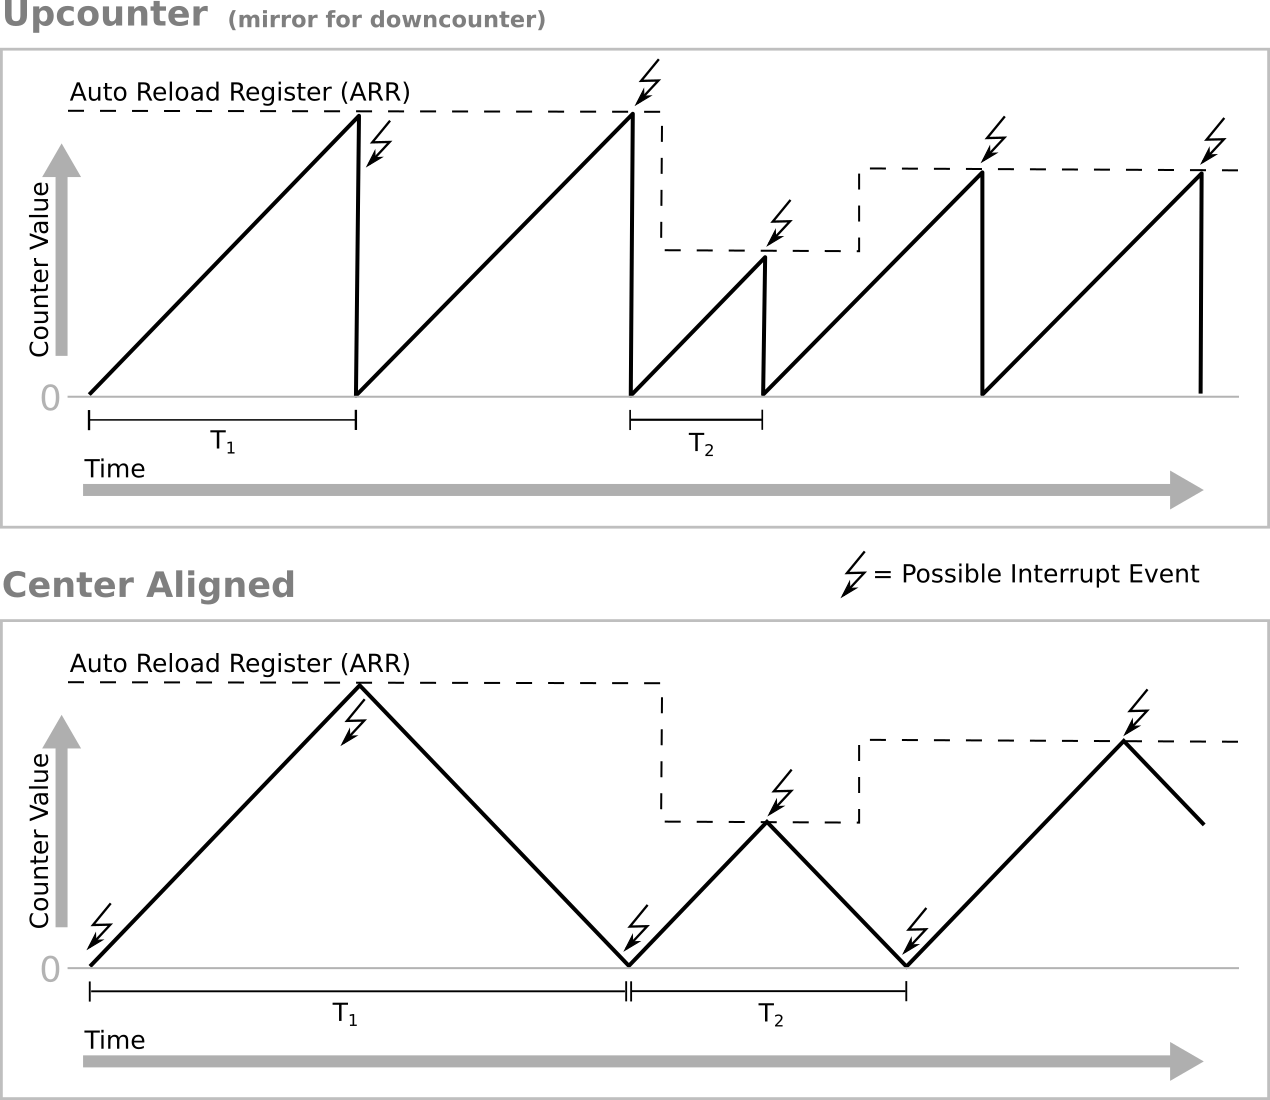
\includegraphics[width=0.75\textwidth]{count_modes}
        \caption{Timer counting modes and update interrupts}
        \label{count_modes}
    \end{figure}
    
    \subsubsection{Basic Timer Interrupts}
    
    Regardless of the counting mode used, whenever the timer reaches a limit and is reset to a new value is called an \textit{Update Event} (UEV). Additionally, center-aligned counters can be configured to trigger update events whenever the timer changes to a specific direction. 
    
    The UEV is one of the possible interrupt sources in a peripheral timer. Typically this interrupt source is used to generate periodic interrupts, but with a very flexible and potentially long duration period.
    
    
    \subsubsection{Configuring Basic Timer Settings}
    In addition to the three main timer registers, there are four control registers used to set timer parameters. These are used to enable the timer, set the counting direction, enable the UEV interrupt, and clear the pending interrupt flag in a handler. 
    
    \begin{itemize}
        \item \textbf{Control Registers 1 \& 2 (CR1 \& CR2)} -- These hold the primary configuration options of the timer. For example, before the timer can operate it must be enabled using the \textit{Counter Enable} (CEN) bit. 
        \item\textbf{DMA/Interrupt Enable Register (DIER)} -- Controls the possible interrupt sources in the timer.
        \item\textbf{Status Register (SR)} -- Contains pending flags that must be cleared in interrupt handlers.
    \end{itemize}

    \subsection{Selecting Timer Frequency and Interrupt Period}	
    The peripheral timers in the STM32F0 have the ability to use a few different sources for their clock input. 
    \begin{itemize}
        \item\textbf{Internal Peripheral Clock} -- This is the most commonly used clock source and is determined by the clock distribution system. In our toolchain, this frequency is configured by default to be 8Mhz by the STMCubeMX program during project generation. 
        \item\textbf{External Clock Pin} -- Many timers have the ability to use an external clock source provided by an input pin. This source may have a unique frequency or higher accuracy than the processor clock.
        \item\textbf{Internal Trigger Inputs} -- Some peripherals can generate trigger events that are visible throughout the device. This mode is used to chain timers together or counting events produced by other types of peripherals.
    \end{itemize}
 
    \subsubsection{Using the Prescaler}
      
        The primary purpose of the timer prescaler is to determine the base unit of time that a single ``tick'' or count within the actual timer represents. Consider a timer operating at 8Mhz, at this frequency the period between each update of the timer's value would be one-eighth of a micro-second or 125ns. While it is possible to use this unit of time as a basis for counting longer periods, it may not be convenient. 
        
        The prescaler allows us to convert the input clock frequency into more practical units. For example, if we wanted to count something with a duration in milliseconds, it would be reasonable to divide the input 8Mhz clock by a factor of 8000, giving us a base unit of 1ms between each timer count. 
        
        Within the timer hardware, the value of the prescaler register (PSC) is 0-indexed. This means that the value written to the PSC register should always be one less than the desired prescaler value. Conveniently this also means that the default value of 0 in the PSC register divides by 1, performing no frequency division on the input clock.  

    \subsubsection{Calculating Register Values}
        Using both the prescaler and auto-reload register makes configuring a timer to have a specific period trivial. First, consider the unit of time that your desired period is in, and use the prescaler to convert the timer's base unit to either the same or a convenient multiple/divisor. Afterward, use the auto-reload register to count the desired number of time units to make the target period. 
        
        If you are attempting to generate a very long period, you may have to use larger or more granular base units because the physical size of the timer may not be sufficient to count that high at a fine resolution. However, in many cases, it is possible to use small prescaler values to have finer granularity when counting.
        The following four equations may be helpful when selecting prescaler and auto-reload values from a target period or frequency. 
        
        %\begin{displaymath}
        \begin{align*}
            & T_{TARGET} = \frac{(PSC-1)}{f_{CLK}} * ARR & & f_{TARGET} = \frac{f_{CLK}}{(PSC-1) * ARR}\\[1em]
            & PSC = \frac{f_{CLK}}{ARR * f_{TARGET}}-1 & & ARR = \frac{f_{CLK}}{(PSC+1) * f_{TARGET}}
        \end{align*}
        %\end{displaymath}
        	
            
        \begin{center}
            \begin{example}[Calculating ARR and PSC Values] 
            For this example, we will set a timer to produce an interrupt at 20Hz assuming that the timer's input clock is 8Mhz. \\
            
            A target frequency of 20Hz gives a 50ms period. To achieve this, we can divide the 8Mhz clock by 8000 to reduce our timer's frequency to 1kHz. Counting at 1kHz gives us 1ms per timer count, so we need 50 counts to reach our target period. We can get our desired interrupt by setting the PSC to 7999, the ARR to 50, and enabling the UEV interrupt in the control registers.  
            \end{example}
        \end{center}
        
    

\section{Using Timers to Generate or Measure Signals}
The basic modes of operation in a timer allow for a very flexible method of generating interrupts by modifying the timer's frequency and top value. However, the timers in the STM32F0 have the additional capability of generating and measuring physical waveforms by directly interfacing with GPIO pins. These features are made possible by the Capture/Compare Unit in the timer. 

When configured in a capture/compare mode, the timer has two additional registers with important functions.  In figure \ref{avaliable_timers} one of the columns indicated how many capture/compare channels were present within each timer. Each capture/compare channel functions independently but has an identical interface with its own set of registers.  
\begin{itemize}
    \item \textbf{Capture/Compare Registers (CCRx)} -- This register hold capture/compare data. Its specific use depends on the selected mode.
    \item \textbf{Capture/Compare Mode Registers (CCMRx)} -- Contains additional options to select between specific capture/compare modes and their operation.
\end{itemize}

The three basic modes that the capture/compare channels can be configured into are input capture mode, output compare mode, and pulse-width modulation mode. Although these modes are primarily intended to interface with their associated GPIO pins, they all can generate interrupts on their respective trigger conditions. 

%    These modes all use the capture/compare circuity of the timer
%    Brief overview of the capture/compare unit
%    
%    The mode of operation of the capture/compare unit is set by the 3 capture/compare mode registers. (CCMR1-3)				
    
    \subsection{Input Capture Mode}
    When configured into input capture mode, a capture/compare channel latches the current value of the timer's counter into the appropriate CCRx register whenever a connected external GPIO pin changes. This mode allows very accurate measurement of the time elapsed between changes on the pin. 
    
    Similar to the EXTI, the input capture hardware can be set to trigger on either the rising or falling edges of a signal. However, the input capture system has a configurable digital filter which can be used to remove glitches and other noise from the signal. The primary purpose of the input capture mode is to measure precise timing-based signals such as those from a single-wire serial bus or a motor encoder.  
%        Keep brief, not focus of lab
%        Basic theory and graphical example		
%        Simple use-cases: stopwatch, tracking motor speed using a click-wheel
%            will be using a fancy version of input capture mode (quadrature encoder mode) to track speed and direction of the motor in later labs.
%        Counter value saved in the capture/compare register (CRR)
    
    \subsection{Output Compare Mode}
        The output compare mode directly modifies the output of a GPIO pin whenever the timer's counter matches the value stored in the CCRx register. Depending on the configuration, an output compare channel can set, clear or toggle its pin on a counter match. 
        
        By using the output compare mode, it is possible to create arbitrary digital waveforms on the output. Typically, the ARR register is set to provide a constant period to the timer, and the user's application produces the desired output by modifying the CCRx register while the timer is running. Figure \ref{ocomp_mode} shows an up-counting timer toggling an output compare pin on every match of the CCRx register.  
        
%        Output compare mode uses an extra control register CCR
%        The timer operates like normally with the counter and ARR but a capture/compare interrupt/event occurs whenever the timer counter reaches the value in the CCR.
%        
%        The capture/compare unit can directly modify the output of a pin on this compare event
%        What happens to the pin (set-high, set-low, toggle) depends on the mode in the control register. 
%        
%        (figure of edge-aligned toggle on match )
        \begin{figure}[]
            \centering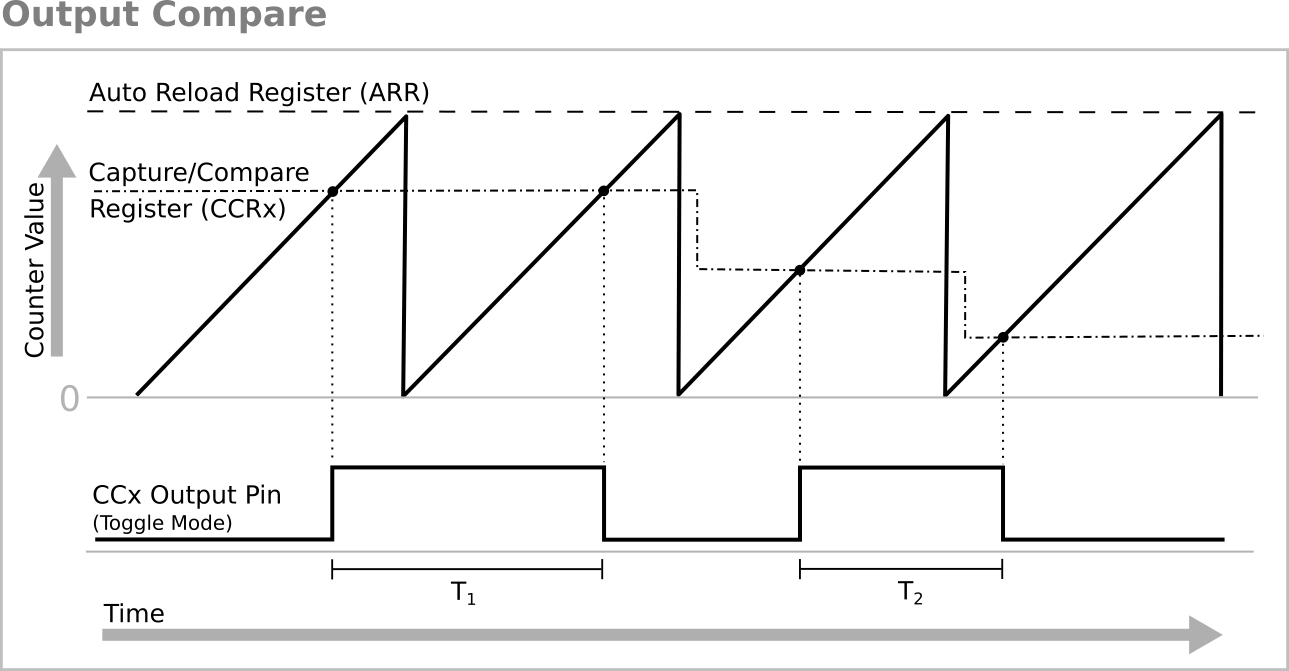
\includegraphics[width=0.75\textwidth]{ocomp_mode}
            \caption{Output Compare mode with pin toggle on compare match.}
            \label{ocomp_mode}
        \end{figure}
    
%        The capture compare mode register can be changed on-the-fly, moving the event point. This is often used in PWM mode.
    
    \subsection{Pulse-Width Modulation (PWM) Mode}
    The pulse-width modulation mode of the capture/compare system is a more advanced form of the output compare mode. However, it is helpful first to discuss pulse-width modulation (PWM) and its uses. 
    
    \subsubsection{About Pulse-Width Modulation}
    PWM is a method of approximating an analog signal using only digital hardware. It operates by using a high-frequency rectangular-wave signal where every period is a ratio of on and off time. This ratio of on/off timing is known as the \textit{duty-cycle} and represents an analog voltage ranging between the low and high voltages of the digital signal. 
    
    For example, a period of the rectangular wave with a 50\% duty cycle would spend half the period at the high (on) output voltage and the other half at the low (off). A period with 0\% duty cycle remains low for the entire duration, and one with a 100\% duty cycle remains high. It is possible to see how the duty cycle of a PWM signal represents an analog voltage by considering what the average voltage of the digital signal was over the entire period. A digital waveform that was high (on) for half the time and off for the rest would average to one-half the original voltage.  
    
    Naturally, the concept of PWM does not make sense at low frequencies; it would just appear as a series of different length flashes. However, at high frequencies, many physical systems cannot respond quick enough to shut-off or turn-on with each output transition. This is the basis of mechanical and electrical low-pass filters which average or smooth out the high-frequency transitions of the PWM signal into an approximated analog signal.
    
    PWM is used for a variety of purposes. A few common examples are audio, light dimming, and motor speed control. Figure \ref{pwm_sine} shows how an analog sine-wave is approximated by a digital PWM signal. 
    
%    What is PWM?
%    What is it used for? How does it approximate an analog signal?
%        low-pass filter
%        electronic, mechanical (motor or speaker), others (human eye)
%        
%    (figure of PWM representing sinewave)
    \begin{figure}[]
        \centering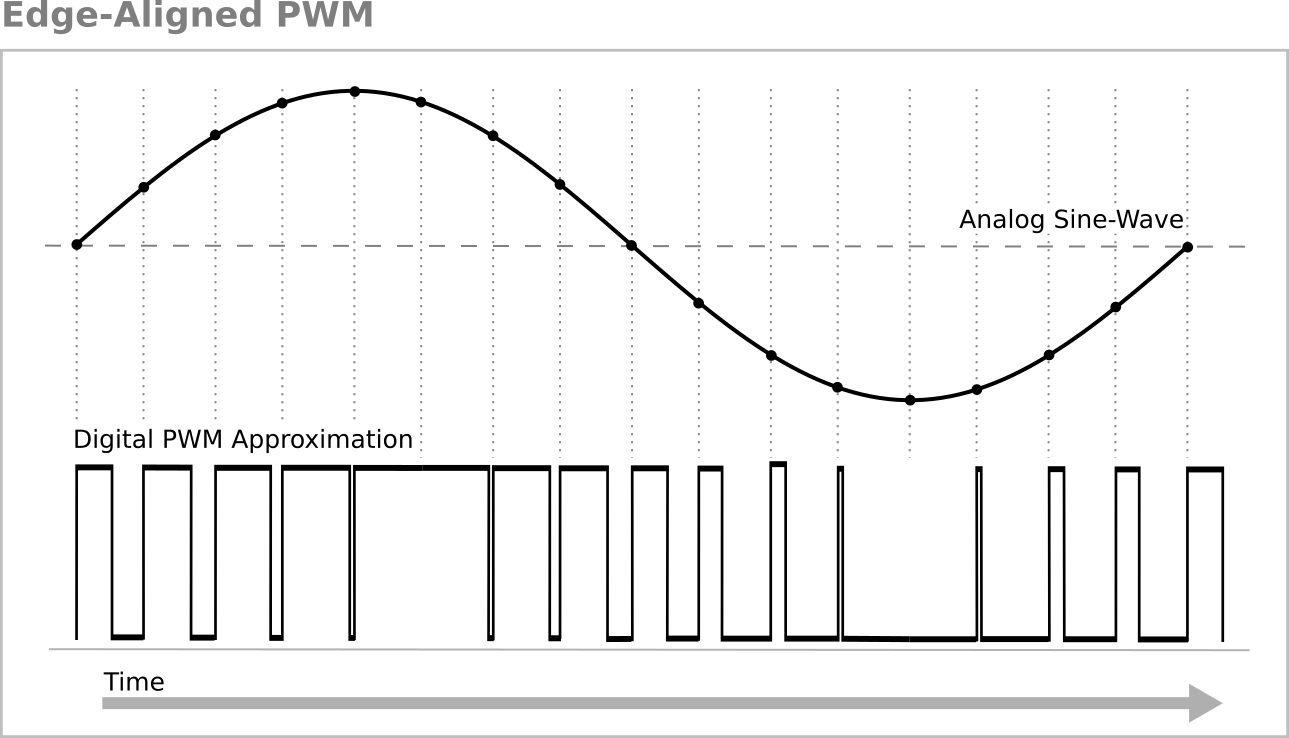
\includegraphics[width=0.75\textwidth]{pwm_sine}
        \caption{PWM approximation of an analog sine-wave.}
        \label{pwm_sine}
    \end{figure}
    
    \subsubsection{Operation of Capture/Compare PWM Mode}
    The PWM mode operates almost exactly to the output compare mode of the timer. The difference is that the output pin state is also modified whenever the timer counter resets to begin a new period. There are different modes of PWM that the capture/compare system can generate. Figure \ref{pwm_pin} demonstrates one of the possible PWM modes. In the mode shown in the figure, the output pin begins the PWM period at a low state and is set high once the timer's counter matches the CCRx register. This output is set low again once the next period starts and the overall ratio of on/off is set by the location of the CCRx value in comparison to the ARR register. 
   
   The important ting to note about PWM is that the signal has both a duty-cycle and frequency. The frequency of the PWM is set by the timer's frequency and the ARR register. The duty-cycle is set by the ratio of the CCRx and ARR registers. Typically the frequency of the PWM signal is irrelevant to the approximated analog voltage. However, it must remain high enough such that the physical low-pass filter smooths out the transitions. 
   
    
    
%    How the STM32F0 generates PWM (fancier form of output compare)
%    Perhaps in list mode where the registers involved are listed with their function?
%    (figure of edge-aligned mode/sawtooth with appropriate markings)
     \begin{figure}[]
        \centering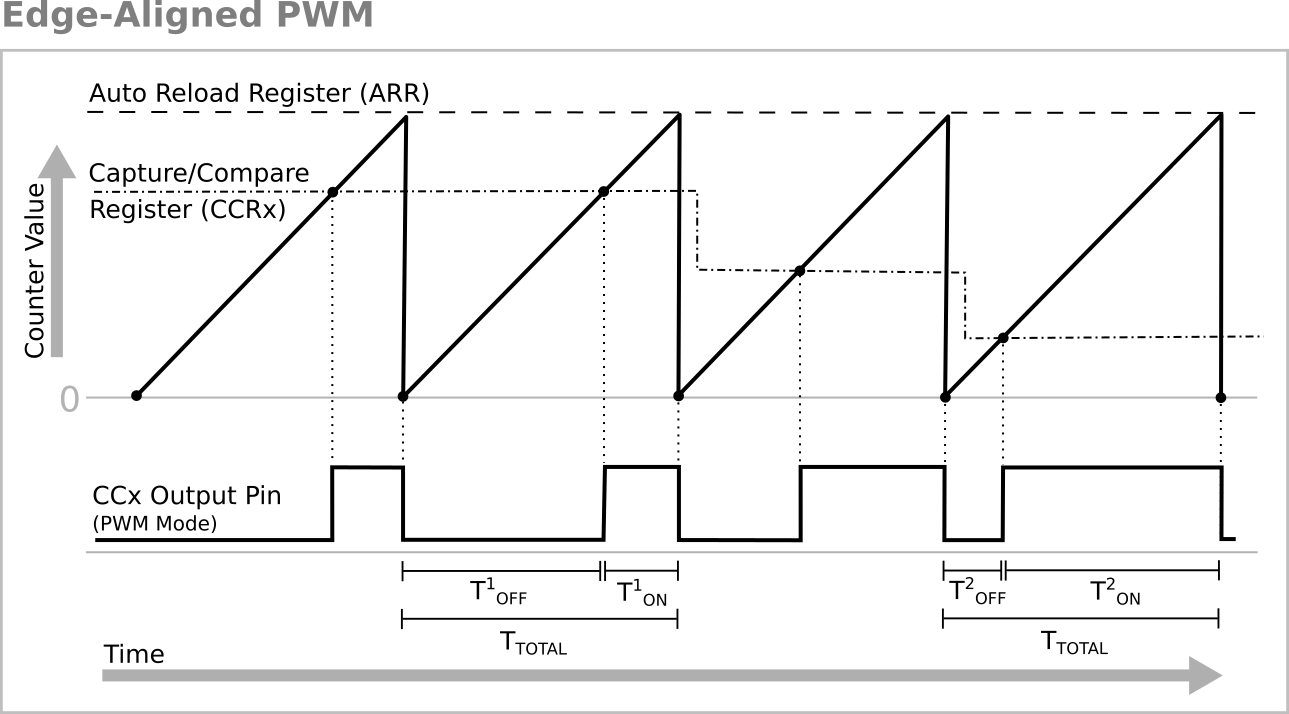
\includegraphics[width=0.75\textwidth]{pwm_pin}
        \caption{Edge-aligned PWM mode and output pin state.}
        \label{pwm_pin}
    \end{figure}

\section{Configuring GPIO pins to Alternate Function Mode} \label{alternate_mode}

Considering that in normal operating conditions a GPIO peripheral controls the output state of its pins, how does another peripheral such as a timer modify a pin's state? The answer lies within one of the available GPIO modes. In the GPIO mode register (MODER) there are four available pin modes, these are Input, Output, Analog and Alternate Function. Allowing a pin to connect directly to internal peripherals of the STM32F0 is the purpose of the alternate function mode. 

Unlike the EXTI which has the SYSCFG multiplexers, peripherals like the timers do not have access to arbitrary pins. Instead, internal signals are hardwired to a limited number of pins scattered around the chip. Many GPIO pins have multiple alternate functions from a variety of peripherals. However, only a single alternate function can be enabled on a pin at a time.

This system allows the user to have a few different options when selecting pins that connect to a peripheral. Because these pins have multiple alternate functions, they are shared across multiple peripherals. When using many peripherals you many need to carefully plan the pins used to ensure that all peripherals can reach one of their limited output pins.  

%    What is Alternate Function Mode?
%    Need to tell the GPIO hardware to allow the timer to directly control the pin output state
%    Connecting a pin to an internal peripheral of the device is called "Alternate Function Mode"
%    In the STM32F0s most peripherals are directly connected to specific sets of pins. 
%        Not like the EXTI which has the SYSCFG muxes to everywhere
%        While you can't assign an internal signal to an arbitrary pin, they do give you a few pin options to choose.
%        Most GPIO pins have multiple possible alternate functions, need to look up. 
%    
%    Use chip datasheet (Pinouts and pin descriptions section)
    
    \subsection{Finding Available Pins on a Device Package}
    
    Alternate function assignments are specific to the STM32F0 device used. This means that the information on pin alternate functions is found within the \textit{device datasheet} and not the peripheral reference manual.
    
    Open the STM32F072xB datasheet and navigate to section 4 \textit{Pinouts and Pin Descriptions}. This section of the datasheet provides documentation on all of the chip packages available for the device. It also provides tables with pinout details, including alternate functions.
    
    Navigate past the package maps until you find table 13 \textit{STM32F072x8/xB pin definitions}. This table provides pin number to pin name mappings, pin characteristics and limitations, and available alternate functions. Figure \ref{chip_pins} shows an annotated subset of table 13. 
    
    \subsubsection{Physical Pin Numbering}
    Beginning from the left-side of the table, the first set of column headers list the different packages available for the chip. These columns provide the physical pin numbering of the chip for that specific package. The STM32F072xB on the Discovery board we are using has a 64-pin low-quad-flat-pack (LQFP64) chip package; this column has been highlighted in orange. Notice that the lowest two rows do not have a number and are highlighted in red, this indicates that the specific pin on that row does not physically exist in the given package. 
    
    \begin{warning}
        When selecting pins, always make sure they exist physically on the device package you are using! All GPIO outputs exist on the silicon die of the STM32F0. However, there aren't enough pins available on every type of chip packaging, and they are not all wired out.
    \end{warning}

    \subsubsection{Pin Name and Characteristics}
    The next column highlighted green and titled ``Pin Name'' gives the conventional pin name indicating the specific GPIO port and location within the peripheral registers. When designing a hardware circuit around an STM32F0 device the information in this table is required to correctly map pin names used in software, to physical pin numbers on the chip. 
   
   The next three columns give information about the input/output circuitry driving the pin. The definitions of the acronyms used are listed in Table 12. 
    
    \subsubsection{Alternate and Additional Functions}
    The blue highlighted ``Alternate Functions'' column lists the various peripheral signals that are available for the specific pin. Once configured into alternate function mode, the GPIO peripheral connects one of these signals. The specific function connected is selected by the GPIO Alternate Function Registers (AFR).
    
    The ``Additional Functions'' column lists pin capabilities connected when the pin is in analog mode. These are discussed in a later lab specifically dealing with the analog peripherals of the STM32F0.


%    Using a 64-pin LQFP (LQFP64)
%    Table 13. STM32F072x8/xB pin definitions
%    Only have pins that have physical pin numbers under the LQFP64 column. Table lists pin assignments for all chip packages the STM32F072 device is produced in.
%    Alternate functions listed, will be talking about other columns of table in later labs.
%    
%    (marked Figure of table 13, package column highlighted, pin name and possible alternate functions)
    \begin{figure}[]
        \centering
\includegraphics[width=0.8\textwidth]{chip_pins}
        \caption{Subset of table 13 - STM32F072x8/xB Datasheet}
        \label{chip_pins}
    \end{figure}

    \begin{example}[Finding Pins With an Alternate Function]
            In this example, we will find a pin that connects to the fourth capture/compare channel of timer 3. Browsing through the alternate functions column in figure \ref{chip_pins} shows the desired function circled in blue. Looking across the row describing the specific pin we can see that this pin belongs to GPIOB (circled in green) and is the 27th physical pin on the LQFP64 package used on the Discovery board (circled in orange).
        
%            Example: Chose arbitrary alternate function for a peripheral and walk through the process of finding pins
    \end{example}
%    (add in section on how to graphically do this with stmcube later)
    
    \subsection{Selecting an Alternate Function}
    Although a pin may have multiple alternate functions, it can only be used for one of them at a given time. Within the GPIO peripherals there are two registers that control what functions are connected to each pin. These are the \textit{Alternate Function High Register} (AFRH) and the  \textit{Alternate Function Low Register} (AFRL). 
    
    Within these registers are regions of bits that select alternate functions by their alternate function number for the pin. These function numbers are documented in tables 14-19 of the \textit{Pinouts and Pin Descriptions} section in the device datasheet. 
%    Demonstrate the AFR registers in the GPIO peripheral
%    Once have pins that can use the AF, need to find what specific AF number it is for that pin.
%    Use tables 14-19 in the chip datasheet
%    
%    (marked figure of table 14-19, pick a GPIO and an alternate function) 

   	
    \begin{example}[Determining an Alternate Function's Number] 
Figure \ref{func_pins} shows a portion of table 15 in the pinouts and pin descriptions section of the device datasheet. This table lists the alternate functions for the GPIOB pins of the device. Continuing from the previous example, we can begin by finding the row representing PB1, the pin chosen with desired alternate function found in Table 13. 

The row representing PB1 has been highlighted in green. Looking across the columns of the row shows the different alternate functions that were also listed in Table 13. Finding the desired alternate function, circled in blue, we can look up to the column header and see the alternate function number circled in red is ``AF1.'' 

By programming the matching bit pattern documented in the AFR register map for ``AF1'' into the bit region representing PB1 in the GPIOB alternate function registers we can select the capture/compare channel 4 of timer 3 to output on that pin.  
%         Example: Find AF number and select for pin in previous example.
    \end{example}

    \begin{figure}[]
    \centering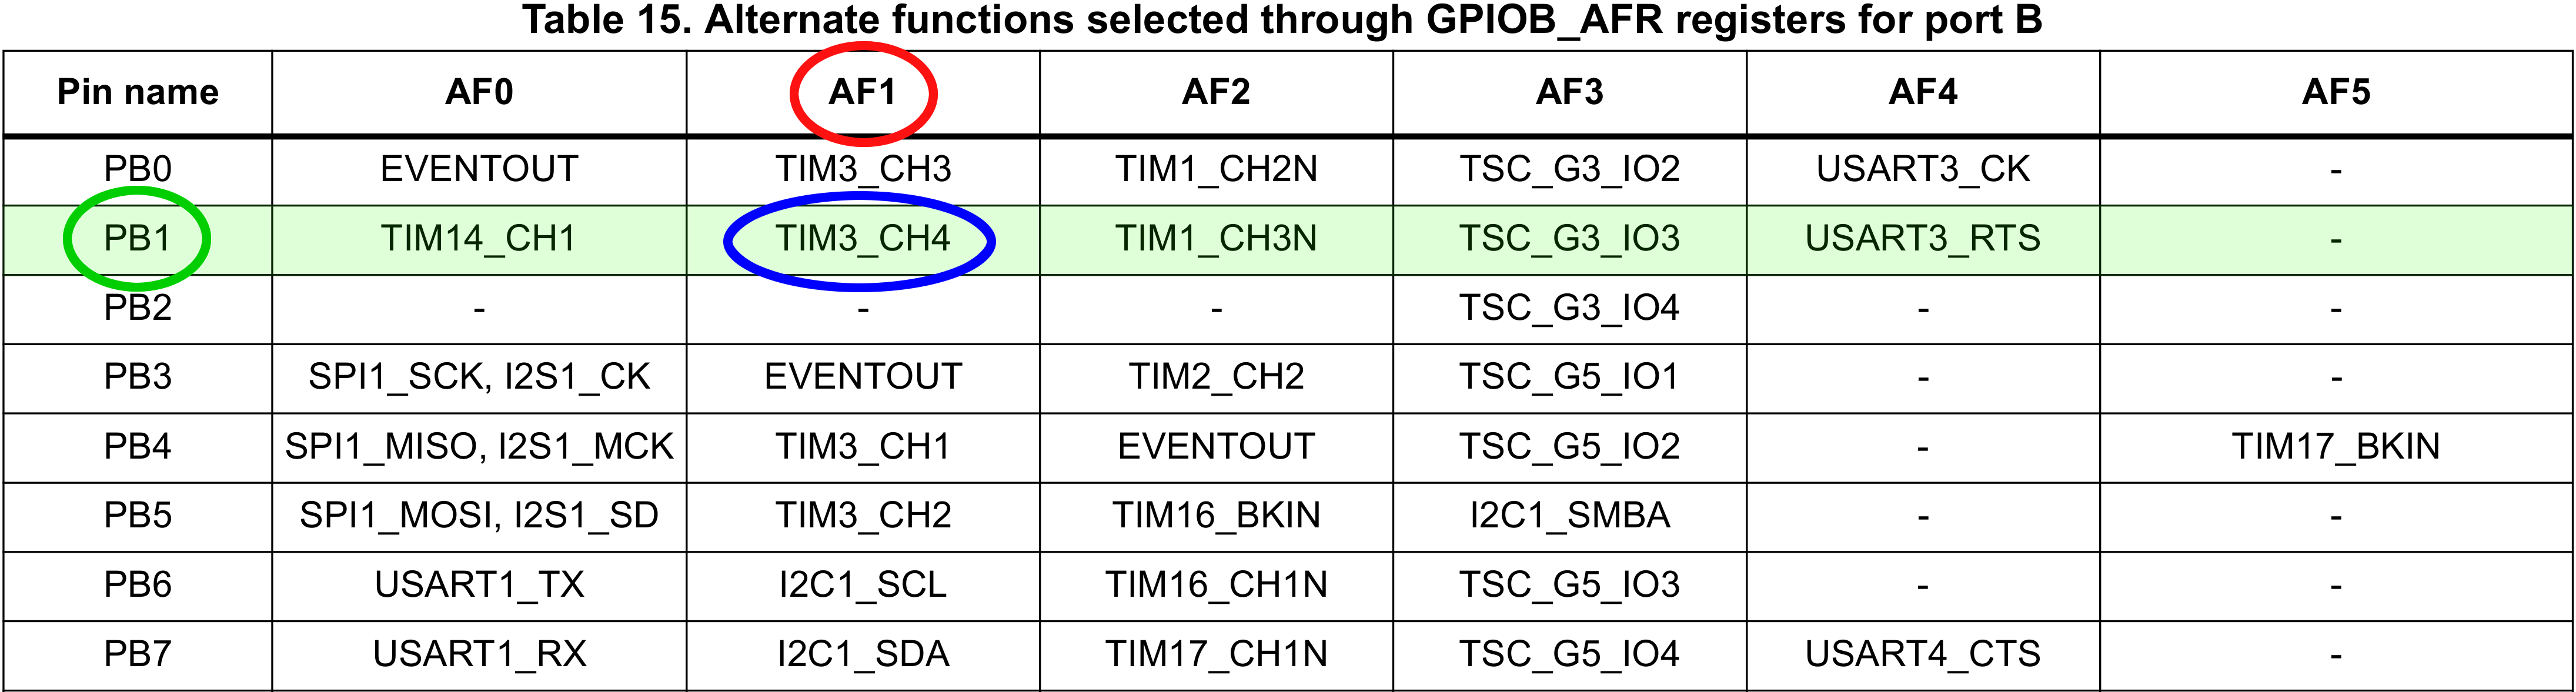
\includegraphics[width=\textwidth]{func_pins}
    \caption{Subset of table 15 - STM32F072x8/xB Datasheet}
    \label{func_pins}
\end{figure}
    
\section{Lab Assignment:}
For these exercises you will be working with one or more timer peripherals in the STM32F0. You are free to use whatever timer you wish for the first portion on timer interrupts. However, since the timers are only routed to a limited selection of pins, you won't have a choice what timers to use for the exercises that generate PWM on  LED pins.  
Because the final exercise combines the two previous ones, you may wish to use the same timer for all three activities. This is possible but requires more thought when choosing timer prescaler and other attributes so that the timer operation is suitable for everything. It is far easier to use two separate timers, one for the longer period interrupt, the other for the short period PWM. 

\subsection{Using a Timer Interrupt}
In this exercise, you'll set up an interrupt such that the update event (UEV) triggers an interrupt at a specific period. Using a timer peripheral allows for much greater flexibility in choosing an interrupt period over manually counting in the SysTick handler. Section \ref{timer_interrupts} provides the background information on how a timer needs to be configured to produce UEV interrupts. However, you will need to carefully read through the control register maps in the peripheral reference manual in order to determine the proper option bits to set. 

\begin{itemize}
    \item Select one of the available timers and enable in the RCC.
    \begin{itemize}
        \item You may wish to jump ahead and find the timer that is connected to the LED pins and avoid using that one. 
        \item Check the alternate functions of the LED pins to determine what timer is connected.
    \end{itemize}
    \item Configure the timer such that it triggers an UEV interrupt at 4 Hz.
    \begin{itemize}
        \item \textbf{The default processor frequency of the STM32F072 is 8 MHz. Use this value when calculating the timer parameters.}
        \item Don't forget to enable the UEV interrupt condition in the timer. 
        \item The timer will only have a single generic interrupt. (not a specific interrupt about the UEV) Look for one named after the timer you are using. 
        \item The timers must be enabled in their control registers before they'll start counting. Don't enable a timer until you've finished setting all the basic parameters and options. 
    \end{itemize}
    \item Do something with two LEDs in the interrupt handler. Leave the other two lights free for the other exercise. 
     \begin{itemize}
         \item Don't forget to clear the UEV pending flag in the timer peripheral. 
     \end{itemize}
     \item Once you have the interrupt running, use a Saleae Logic to measure the period between LED toggles.
     \begin{itemize}
         \item Verify that the measured period is similar to what was expected. (Won't be exact due to context switch overhead, instruction execution etc.)
         \item Include the measured value in your postlab.
     \end{itemize}
\end{itemize}


\subsection{Generating PWM with a Capture/Compare Unit}
In this exercise you will set up PWM output to dim a LED on the discovery board. By changing the duty-cycle of the generated waveform you can directly control the apparent brightness of the LED. For this exercise you will need to find the specific timer and capture/compare channels that connect to the unused LED pins. 

The lab manual mentioned that the frequency of a PWM signal isn't nearly as important as the duty-cycle, provided that the frequency is high enough that the system can't directly respond to the on-off periods. This is true when dimming LEDs, although the lower-limit isn't how fast the LED can respond to the electrical signal, but how fast the human eye can distinguish separate blinks of the LED apart from each other.
When both the light and viewer are stationary, the human eye has difficulty seeing the blinking transitions past 70 Hz. However, many people can see noticeable flicker in moving lights even above 500 Hz. Because of this, you'll be using 800 Hz as the base frequency for the PWM. 

\begin{itemize}
    \item Find the timer that has its capture/compare channels connected to the unused LEDs. 
    \item Configure the LED pins in the GPIO peripheral to alternate function mode, and select the timer's capture/compare alternate function.
    \item Configure the timer to have a UEV period of 800 Hz, but \underline{don't} enable the UEV interrupt. (not using the interrupt)  
    \begin{itemize}
        \item Set the prescaler such that you have a reasonable range of counter values between zero and the top limit. 
        \item Otherwise your timer will be too granular to be able to make fine adjustments to the duty-cycle of the PWM.
    \end{itemize}
    
    \item Configure the appropriate capture/compare channels that connect to the LED pins to \underline{\textit{PWM mode 1}}. 
    \item Set the capture/compare register to the following values and observe the results using a logic analyzer:
    \begin{itemize}
        \item 25\% the value of the ARR register
        \item 50\% the value of the ARR register
        \item 75\% the value of the ARR register
    \end{itemize}
    \item Make sure to note the general behavior and change in duty-cycle for your postlab.
    \item Change the capture/compare channels connecting to the LED pins to \underline{\textit{PWM mode 2}}.  
    \begin{itemize}
        \item Repeat the same steps performed above with the new mode.
    \end{itemize}   
    \item Take a screenshot of one of the logic captures and include in your postlab. 
\end{itemize}


\subsection{Building an LED Crossfader}
This final exercise uses the concepts of both the previous experiments to build a fun example. In this section, you'll set up two LEDs such that one of them will fade dimmer over time, while the other fades brighter. Once the limits have been hit, the direction will reverse and repeat. 

\begin{itemize}
    \item Set up the timer and GPIO to PWM two LEDs.
    \item Set up a longer-period timer interrupt. (the one used in the first experiment is fine)
    \item Set the PWM duty-cycles so that one LED is bright and the other is off.
    \item Incrementally modify the PWM duty-cycles in the timer interrupt, such that the brightness of both LEDs fade in opposite directions. 
    \begin{itemize}
        \item Once the end limits have been reached, reverse the direction
        \item You can either keep separate variables tracking the direction and value of each capture/compare channel, or set the PWM modes such that only a single value is necessary.
    \end{itemize}
\end{itemize}
 

\end{document}
